\documentclass[12pt]{article}

\usepackage[margin=1in]{geometry}
\usepackage{amsmath,amsthm,amssymb}
\usepackage{nccmath}
\usepackage{mathtools}
\usepackage{mathrsfs}
\usepackage{enumitem}
\usepackage{physics}
\usepackage{tensor}

\usepackage{tikz}
\usetikzlibrary{calc,decorations.markings,patterns}

\newcommand{\magsq}[1]{\big|#1\big|^2}
\newcommand{\avg}[1]{\left<#1\right>}
\newcommand{\fullint}{\int_{-\infty}^\infty}
\newcommand{\fullintd}[1]{\fullint\dd#1\:}
\newcommand{\cint}[2]{\int_{#1}^{#2}}
\newcommand{\cintd}[3]{\cint{#1}{#2}\dd#3\:}
\newcommand{\boostXY}{\mqty(\gamma & -\gamma\beta_x & -\gamma\beta_y & 0 \\ -\gamma\beta_x & 1 + (\gamma - 1)\frac{\beta_x^2}{\abs{\beta}^2} & (\gamma - 1)\frac{\beta_x\beta_y}{\abs{\beta}^2} & 0 \\ -\gamma\beta_y & (\gamma - 1)\frac{\beta_x\beta_y}{\abs{\beta}^2} & 1 + (\gamma - 1)\frac{\beta_y^2}{\abs{\beta}^2} & 0 \\ 0 & 0 & 0 & 1)}
\newcommand{\metric}{\mqty(1 & 0 & 0 & 0 \\ 0 & -1 & 0 & 0 \\ 0 & 0 & -1 & 0 \\ 0 & 0 & 0 & -1)}

\begin{document}

\title{Homework 1}
\author{Sean Ericson \\ Phys 661}
\maketitle

\section*{Problem 1}
\begin{enumerate}[label=(\alph*)]
    \item 
        \[ 
            \mqty(t' \\ x' \\ y' \\ z') = 
            \mqty(
                \gamma_x & -\gamma_x V_x & 0 & 0 \\
                -\gamma_x V_x & \gamma_x & 0 & 0 \\
                0 & 0 & 1 & 0 \\
                0 & 0 & 0 & 1
            )
            \mqty(t \\ x \\ y \\ z)
        \]

    \item
        \[ 
            \mqty(t' \\ x' \\ y' \\ z') = 
            \mqty(
                \mu & \nu & 0 & 0 \\
                \sigma & \gamma & 0 & 0 \\
                0 & 0 & \rho & 0 \\
                0 & 0 & 0 & \lambda
            )
            \mqty(t \\ x \\ y \\ z)
        \]
\end{enumerate}


\section*{Problem 2}
\begin{align*}
    \mqty(t' \\ x' \\ y' \\ z') &= 
        \mqty(
            \gamma_y & 0 & \gamma_y V_y & 0 \\
            0 & 1 & 0 & 0 \\
            \gamma_y V_y & 0 & \gamma_y & 0 \\
            0 & 0 & 0 & 1
        )
        \mqty(
            \gamma_x & \gamma_x V_x & 0 & 0 \\
            \gamma_x V_x & \gamma_x & 0 & 0 \\
            0 & 0 & 1 & 0 \\
            0 & 0 & 0 & 1
        )
        \mqty(
            \gamma_y & 0 & -\gamma_y V_y & 0 \\
            0 & 1 & 0 & 0 \\
            -\gamma_y V_y & 0 & \gamma_y & 0 \\
            0 & 0 & 0 & 1
        )
        \mqty(
            \gamma_x & -\gamma_x V_x & 0 & 0 \\
            -\gamma_x V_x & \gamma_x & 0 & 0 \\
            0 & 0 & 1 & 0 \\
            0 & 0 & 0 & 1
        )
        \mqty(t \\ x \\ y \\ z) \\
    &= \mqty(
        -\gamma_x^2\gamma_y^2 \left(\frac{V_x^2}{\gamma_y^2} + \frac{V_y^2}{\gamma_x^2} - 1 \right) & \gamma_x^2\gamma_y^2V_x\left(\frac{V_y^2}{\gamma_x} + \frac{1}{\gamma_y} - 1\right) & -(\gamma_x - 1)\gamma_y^2V_y & 0 \\
        (\gamma_y - 1)\gamma_x^2V_x & \gamma_x^2\left(1 - \gamma_yV_x^2\right) & -\gamma_x\gamma_yV_xV_y & 0 \\
        -\gamma_x^2\gamma_y^2V_y\left(\frac{V_x^2}{\gamma_y} + \frac{1}{\gamma_x} - 1\right) & \gamma_x^2\gamma_y^2V_xV_y\left(\frac{1}{\gamma_x} + \frac{1}{\gamma_y} - 1\right) & -\gamma_y^2\left(\gamma_xV_y^2 - 1\right) & 0 \\
        0 & 0 & 0 & 1
        )
        \mqty(t \\ x \\ y \\ z)
\end{align*}
Composing the four given boosts results in the more complicated lorentz transformation given above. This transformation is not symmetric, so it's clearly not a pure boost. It leaves the $z$-component untouched, so it must be a combination of a boost in the $xy$-plane and a rotation about the $z$-axis (or vice-versa). \\
Expanding this to lowest order in $V_x$ and $V_y$ (using Mathematica), I found that this transformation is just the identity, with corrections that are second-order in the $V$s.

\section*{Problem 3}
\begin{enumerate}[label=(\alph*)]
    \item From the frame of the Earth, the photon is traveling towards the origin, making an angle $\theta$ with the $z$-axis, as shown in Figure \ref{fig1}. In a time $\Delta t$, the photon travels a distance $\Delta t$ ($c$ = 1). Its $x$-displacement is therefore $\Delta x = -\Delta t \sin\theta$, while the $z$-displacement is $\Delta z = -\Delta t \cos\theta$.
    \begin{figure}
        \centering
        \resizebox{250pt}{!}{
            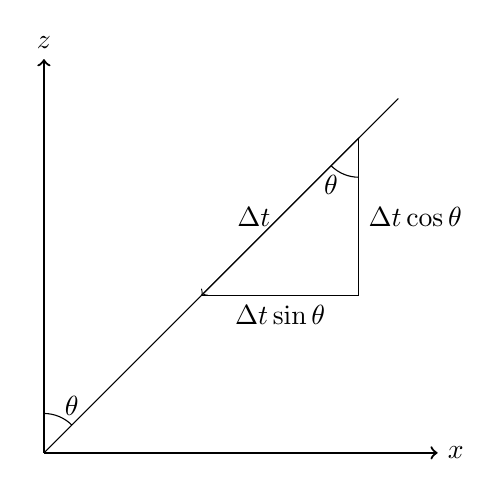
\begin{tikzpicture}
                % Axes
                \draw[->, thick] (0,0)--(0,5) node[above]{$z$};
                \draw[->, thick] (0,0)--(5,0) node[right]{$x$};

                % incoming ray
                \draw (4.5,4.5)--(0,0);
                \draw (0, 0.5) arc (90:45:0.5) node[above]{$\theta$};

                % triangle
                \draw (4,4)--(4,2) node[midway,right]{$\Delta t \cos\theta$};
                \draw (2,2)--(4,2) node[midway,below]{$\Delta t \sin\theta$};
                \draw[->] (4,4)--(2,2) node[midway,above,left]{$\Delta t$};
                \draw (4, 3.5) arc (270:225:0.5) node[below]{$\theta$};
            \end{tikzpicture}
        }
        \caption{The photon's path in the $xz$-plane.}
        \label{fig1}
    \end{figure}
    \item Using the transformation for a boost along the $z$-direction,
        \begin{align*}
            t' &= \gamma t - \gamma V z \\
            x' &= x \\
            y' &= y \\
            z' &= \gamma z - \gamma V t,
        \end{align*}
        we can transform the displacement 4-vector to the ship's frame:
        \begin{align*}
            \Delta t' &= \gamma\Delta t - \gamma V \Delta t \sin\theta \\
            & = -\gamma\Delta t(V + \cos\theta) \\
            \Delta x' & = \Delta x \\
            \Delta y' &= \Delta y \\
            \Delta z' &= -\gamma\Delta t \cos\theta - \gamma V \Delta t \\
            &= -\gamma \Delta t (1 + V\cos\theta).
        \end{align*}
        An observer from the ship could draw the exact same diagram as Figure \ref{fig1} (with $\theta \to \overline{\theta}$), so the ship-based observer can calculate $\cos\overline{\theta}$ as $\Delta z' / \Delta t'$, thus
        \[ \cos\overline{\theta} = \frac{\Delta z'}{\Delta t'} = \frac{V + \cos\theta}{1 + V\cos\theta} \]
    \item 
        \begin{alignat*}{2}
             \quad &\theta = \frac{\pi}{2} \\
            \implies & \cos\theta = 0 \\
            \implies & \cos\overline{\theta} = \frac{V + 0}{1 + 0} = V \\
            \implies & \overline{\theta} = \cos^{-1}V
        \end{alignat*}
        If $V = 0.9c$, this gives a $\overline{\theta}$ of about 0.45 rad ($~25.8^\circ$), while for $V = 0.99c$ this gives about 0.14 rad ($~8^\circ$).
    \item 
        \begin{alignat*}{3}
            &         \quad &\cos\overline{\theta} &= \frac{V + \cos\theta}{1 + V\cos\theta} \\
            &\implies \quad &  1 - \frac{1}{2}\overline{\theta}^2  &\approx \frac{V + 1 - \frac{1}{2}\theta^2}{1 + V - \frac{1}{2}V\theta^2}  \\
            &\implies \quad & \quad &\approx (V + 1 - \frac{1}{2}\theta^2)\left(\frac{1}{1 + V} + \frac{\frac{1}{2}V\theta^2}{(1 + V)^2}\right) \\
            &\implies \quad & \quad &\approx 1 + \frac{\frac{1}{2}V\theta^2}{V + 1} - \frac{\frac{1}{2}\theta^2}{V + 1} \\
            &\implies \quad & -\overline{\theta}^2 &\approx \frac{V - 1}{V + 1}\theta^2 \\
            &\implies \quad & \overline{\theta} &\approx \sqrt{\frac{1 - V}{1 + V}}\theta \\
        \end{alignat*}
\end{enumerate}

\end{document}